\PassOptionsToPackage{table}{xcolor}
\documentclass[11pt,a4paper]{article}

% ==============================================================================
% PACKAGES & GEOMETRY
% ==============================================================================
\usepackage[a4paper,margin=1.8cm,headheight=26pt,top=2.2cm,bottom=2.0cm]{geometry}
\usepackage{fontspec}
\usepackage{amsmath,amssymb}
\usepackage{enumitem}
\setlist{nosep,leftmargin=1.4em,topsep=2pt,itemsep=2pt}
\usepackage{booktabs}
\usepackage{colortbl}
\usepackage{tabularx}
\usepackage{array}
\usepackage{tikz}
\usetikzlibrary{shapes,backgrounds,arrows.meta,positioning,calc}
\usepackage{xcolor}
\usepackage[most]{tcolorbox}
\tcbuselibrary{skins,breakable}
\usepackage{fancyhdr}
\usepackage{titlesec}
\usepackage{titletoc}

% Styled Table of Contents
\titlecontents{section}[0pt]
  {\addvspace{4pt}\bfseries\small\color{navy}}
  {\contentslabel[\thecontentslabel]{1.8em}}
  {}
  {\titlerule*[0.5pc]{\color{gray!60}.}\bfseries\color{teal}\contentspage}

\titlecontents{subsection}[2.2em]
  {\addvspace{1pt}\normalfont\footnotesize\color{darkslate}}
  {\contentslabel[\thecontentslabel]{2.2em}}
  {}
  {\titlerule*[0.5pc]{\color{gray!35}.}\color{teal!80!black}\contentspage}

\usepackage[colorlinks=true,linkcolor=teal,urlcolor=teal,citecolor=navy]{hyperref}

% ==============================================================================
% COLOR PALETTE (Navy / Teal / Gold / Coral)
% ==============================================================================
\definecolor{navy}{HTML}{0B2545}
\definecolor{teal}{HTML}{147D75}
\definecolor{gold}{HTML}{C9A227}
\definecolor{lightteal}{HTML}{E7F3F2}
\definecolor{lightgold}{HTML}{FBF3DD}
\definecolor{coral}{HTML}{C0392B}
\definecolor{lightcoral}{HTML}{FDEDEC}
\definecolor{darkslate}{HTML}{1E293B}

% ==============================================================================
% TCOLORBOX ENVIRONMENTS
% ==============================================================================
\newtcolorbox{defbox}[1][Definition]{
  colback=lightteal, colframe=teal, coltitle=white,
  fonttitle=\bfseries\small, colbacktitle=teal,
  title={#1},
  breakable, boxrule=0.8pt, arc=3pt,
  left=8pt, right=8pt, top=6pt, bottom=6pt,
  before skip=6pt, after skip=6pt
}

\newtcolorbox{examplebox}[1][Concrete Example]{
  colback=lightgold, colframe=gold, coltitle=navy,
  fonttitle=\bfseries\small, colbacktitle=lightgold,
  title={#1},
  breakable, boxrule=0.8pt, arc=3pt,
  left=8pt, right=8pt, top=6pt, bottom=6pt,
  before skip=6pt, after skip=6pt
}

\newtcolorbox{theorembox}[1][Proof \& Derivation]{
  colback=white, colframe=navy, coltitle=white,
  fonttitle=\bfseries\small, colbacktitle=navy,
  title={#1},
  breakable, boxrule=1pt, arc=3pt,
  left=8pt, right=8pt, top=6pt, bottom=6pt,
  before skip=6pt, after skip=6pt
}

\newtcolorbox{warningbox}[1][Beginner Trap \& Pitfall Alert]{
  colback=lightcoral, colframe=coral, coltitle=white,
  fonttitle=\bfseries\small, colbacktitle=coral,
  title={#1},
  breakable, boxrule=0.9pt, arc=3pt,
  left=8pt, right=8pt, top=6pt, bottom=6pt,
  before skip=6pt, after skip=6pt
}

\newtcolorbox{notebox}[1][Key Takeaway / Summary]{
  colback=navy!5, colframe=navy!70, coltitle=white,
  fonttitle=\bfseries\small, colbacktitle=navy!70,
  title={#1},
  breakable, boxrule=0.7pt, arc=3pt,
  left=8pt, right=8pt, top=6pt, bottom=6pt,
  before skip=6pt, after skip=6pt
}

\newtcolorbox{exambox}[1]{
  colback=white, colbacklower=teal!6, colframe=navy!90, coltitle=white,
  fonttitle=\bfseries\small, colbacktitle=navy!90,
  title={#1},
  breakable, boxrule=0.9pt, arc=3pt,
  left=8pt, right=8pt, top=6pt, bottom=7pt,
  before skip=6pt, after skip=6pt,
  lower separated=true, borderline horizontal={0.6pt}{0pt}{gold}
}
% Q/A label helpers for consistent, distinguishable exam boxes
\newcommand{\Qlabel}{\textbf{\color{navy}\footnotesize\MakeUppercase{Question}}\par\smallskip}
\newcommand{\Alabel}{\textbf{\color{teal}\footnotesize\MakeUppercase{Answer}}\par\smallskip}

% ==============================================================================
% HEADER & FOOTER
% ==============================================================================
\pagestyle{fancy}
\fancyhf{}
\renewcommand{\headrulewidth}{0.8pt}
\renewcommand{\headrule}{\hbox to\headwidth{\color{teal}\leaders\hrule height \headrulewidth\hfill}}
\renewcommand{\footrulewidth}{0.4pt}
\fancyhead[L]{\small\bfseries\color{navy} CSE 1143: Discrete Mathematics}
\fancyhead[R]{\small\bfseries\color{teal} Propositional Logic}
\fancyfoot[L]{\footnotesize\color{gray} Suleman Ahmed Shuvo}
\fancyfoot[R]{\footnotesize\bfseries\color{navy} Page \thepage}

% ==============================================================================
% SECTION TITLES
% ==============================================================================
\titleformat{\section}
  {\bfseries\Large\color{navy}}
  {\thesection}{0.5em}{}[{\color{gold}\titlerule[1.2pt]}]
\titleformat{\subsection}
  {\bfseries\large\color{teal}}
  {\thesubsection}{0.5em}{}
\titleformat{\subsubsection}
  {\bfseries\normalsize\color{darkslate}}
  {\thesubsubsection}{0.5em}{}

\setlength{\parindent}{0pt}
\setlength{\parskip}{4pt}

\begin{document}

% ==============================================================================
% PUBLICATION COVER PAGE
% ==============================================================================
\begin{titlepage}
\thispagestyle{empty}
\begin{tikzpicture}[remember picture, overlay]
  % Left side color bands
  \fill[navy] (current page.north west) rectangle ($(current page.south west)+(1.2cm, 0)$);
  \fill[teal] ($(current page.north west)+(1.2cm, 0)$) rectangle ($(current page.south west)+(1.5cm, 0)$);
  \fill[gold] ($(current page.north west)+(1.5cm, 0)$) rectangle ($(current page.south west)+(1.65cm, 0)$);
  
  % Top-right decorative geometric corner
  \fill[lightteal, opacity=0.5] ($(current page.north east)+(-6cm, 0)$) -- (current page.north east) -- ($(current page.north east)+(0, -4cm)$) -- cycle;
\end{tikzpicture}

\vspace*{0.8cm}
\begin{flushleft}
\hspace*{0.8cm}
\begin{minipage}{0.88\textwidth}
  {\color{teal}\bfseries\small\MakeUppercase{Discrete Mathematics Study Handbook}}\\[0.6cm]
  {\color{navy}\bfseries\fontsize{26}{32}\selectfont Propositional Logic}
  
  \vspace{1.8cm}
  
  % Center decorative logic implication / equivalence motif
  \begin{center}
  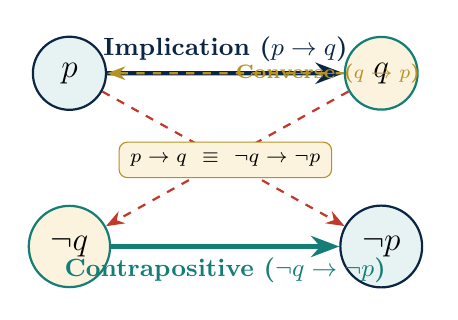
\begin{tikzpicture}[scale=1.1, >=Stealth]
    % Nodes
    \node[circle, draw=navy, fill=lightteal, thick, inner sep=6pt, font=\bfseries\large] (p) at (0, 2) {$p$};
    \node[circle, draw=teal, fill=lightgold, thick, inner sep=6pt, font=\bfseries\large] (q) at (3.6, 2) {$q$};
    \node[circle, draw=teal, fill=lightgold, thick, inner sep=5pt, font=\bfseries\large] (nq) at (0, 0) {$\neg q$};
    \node[circle, draw=navy, fill=lightteal, thick, inner sep=5pt, font=\bfseries\large] (np) at (3.6, 0) {$\neg p$};
    
    % Implication Arrows
    \draw[->, ultra thick, navy] (p) -- node[above, font=\bfseries\small] {Implication ($p \to q$)} (q);
    \draw[->, ultra thick, teal] (nq) -- node[below, font=\bfseries\small] {Contrapositive ($\neg q \to \neg p$)} (np);
    
    \draw[->, thick, dashed, gold!90!black] (q) -- node[right, font=\bfseries\scriptsize] {Converse ($q \to p$)} (p);
    \draw[->, thick, dashed, coral] (p) -- node[left, font=\bfseries\scriptsize] {Inverse} (np);
    \draw[->, thick, dashed, coral] (q) -- node[right, font=\bfseries\scriptsize] {Inverse} (nq);
    
    % Center Equivalence badge
    \node[draw=gold!90!black, fill=lightgold, rounded corners=3pt, font=\bfseries\scriptsize, inner sep=4pt] at (1.8, 1) {$p \to q \ \equiv \ \neg q \to \neg p$};
  \end{tikzpicture}
  \end{center}
  
  \vspace{1.6cm}
  
  % Metadata Card
  \begin{tcolorbox}[
    enhanced,
    colback=white,
    colframe=navy!30,
    boxrule=0.8pt,
    arc=4pt,
    left=16pt, right=16pt, top=14pt, bottom=14pt,
    shadow={2pt}{-2pt}{0pt}{black!10}
  ]
    \renewcommand{\arraystretch}{1.3}
    \begin{tabularx}{\linewidth}{@{}l X@{}}
      \textbf{\color{navy}\small COMPILED BY:} & {\large\bfseries\color{navy} Suleman Ahmed Shuvo} \\
      \textbf{\color{navy}\small ACADEMIC ID:} & {\small\color{darkslate} Roll: 43 \ $\bullet$ \ Batch: CSE-19 \ $\bullet$ \ Session: 2025--2026} \\
      \textbf{\color{navy}\small COURSE:} & {\small\color{teal}\bfseries CSE 1143: Discrete Mathematics (3.00 Credits)} \\
      \textbf{\color{navy}\small DEPARTMENT:} & {\small Dept. of Computer Science \& Engineering} \\
      \textbf{\color{navy}\small INSTITUTION:} & {\small\bfseries Sylhet Engineering College (SEC)} \\
      & {\footnotesize Affiliated with Shahjalal University of Science \& Technology (SUST)} \\
    \end{tabularx}
  \end{tcolorbox}
\end{minipage}
\end{flushleft}
\end{titlepage}

% ==============================================================================
% SYLLABUS GUIDE & TABLE OF CONTENTS
% ==============================================================================
\newpage
\begin{tcolorbox}[
    enhanced,
    colback=lightteal,
    colframe=teal,
    boxrule=0.8pt,
    arc=3pt,
    left=8pt, right=8pt, top=5pt, bottom=5pt
]
\textbf{\color{navy}\normalsize $\bigstar$ SEC TT-01 Tutorial Test Syllabus Guide}\\[2pt]
{\footnotesize\textbf{\color{teal}Tutorial Test Date: 7 September, 2026} $\bullet$ \textbf{Dept. of Computer Science \& Engineering}}\\[2pt]
{\footnotesize Topics marked with a star (\textbf{\color{gold!90!black}$\bigstar$}) are explicitly tested in your TT-01 curriculum: \textit{Proposition, Compound Proposition, Conjunction, Disjunction, Conditional, Converse, Inverse, Contrapositive, Truth Tables, Tautology/Contradiction/Contingency, Logical Equivalences, and Rules of Inference}.}
\end{tcolorbox}
\vspace{6pt}

\begin{center}
{\color{navy}\bfseries\large\MakeUppercase{Table of Contents}}\\[-4pt]
{\color{gold}\rule{\linewidth}{1pt}}
\end{center}
\vspace{2pt}

\begingroup
\hypersetup{linkcolor=navy}
\setcounter{tocdepth}{2}
\makeatletter
\@starttoc{toc}
\makeatother
\endgroup

\newpage

% ==============================================================================
% MODULE 1: THE FOUNDATIONS OF PROPOSITIONAL LOGIC
% ==============================================================================
\section{The Foundations of Propositional Logic}

\subsection{\texorpdfstring{$\bigstar$ }{*}Definition of a Proposition}
Logic is the foundation of mathematical reasoning and computer science. In computing, circuits operate on binary logic gates, conditional control structures evaluate Boolean assertions, and formal algorithms rely on provable logical correctness.

\begin{defbox}[Formal Definition: Proposition]
A \textbf{proposition} is a declarative sentence that is either \textbf{True (T)} or \textbf{False (F)}, but not both simultaneously.
\begin{itemize}
    \item The truth value of a proposition is denoted by $\mathbf{T}$ (or $1$) if it is true, and $\mathbf{F}$ (or $0$) if it is false.
    \item Propositional variables are customarily represented by lower-case letters: $p, q, r, s, \dots$
    \item The area of logic dealing with propositions is known as \textbf{Propositional Logic} (or \textit{Propositional Calculus}, \textit{Sentential Logic}).
\end{itemize}
\end{defbox}

\subsection{Propositions vs. Non-Propositions}
To determine whether an arbitrary sentence is a proposition, test whether it satisfies two criteria:
\begin{enumerate}
    \item It must be a \textbf{declarative} grammatical sentence (it declares a factual assertion).
    \item It must have a definitive truth value ($\mathbf{T}$ or $\mathbf{F}$), independent of opinion, perspective, or unassigned variables.
\end{enumerate}

\begin{examplebox}[Concrete Illustrations of Propositions]
\begin{itemize}
    \item \textit{``Sylhet is a divisional city of Bangladesh.''} $\longrightarrow$ Declarative, factually correct $\implies$ \textbf{Proposition (T)}.
    \item \textit{``$2 + 3 = 7$''} $\longrightarrow$ Declarative mathematical assertion, false $\implies$ \textbf{Proposition (F)}.
    \item \textit{``$\sqrt{2}$ is an irrational number.''} $\longrightarrow$ Declarative mathematical fact $\implies$ \textbf{Proposition (T)}.
    \item \textit{``$2$ is the only even prime number.''} $\longrightarrow$ Declarative, true $\implies$ \textbf{Proposition (T)}.
\end{itemize}
\end{examplebox}

\begin{warningbox}[Sentence Types That Are NEVER Propositions]
\begin{enumerate}
    \item \textbf{Interrogative Sentences (Questions):} \textit{``What is your name?''}, \textit{``Is it raining?''} (Cannot be true or false).
    \item \textbf{Imperative Sentences (Commands / Requests):} \textit{``Read chapter one.''}, \textit{``Please close the door.''}
    \item \textbf{Exclamatory Sentences:} \textit{``What a wonderful goal!''}
    \item \textbf{Self-Referential Paradoxes:} \textit{``This statement is false.''} (If true, then it is false; if false, then it is true).
\end{enumerate}
\end{warningbox}

\newpage

\subsection{Variables in Mathematical Expressions}
A common exam trap involves mathematical expressions containing unspecified variables.

\begin{examplebox}[Variable Truth Dependency]
\begin{itemize}
    \item $1 + 1 = 2$ $\longrightarrow$ No variables; always true $\implies$ \textbf{Proposition (T)}.
    \item $x + 1 = 2$ $\longrightarrow$ Truth value depends entirely on the numerical value of $x$. Without assigning $x$, it is neither true nor false $\implies$ \textbf{Not a Proposition} (it is an \textit{open sentence} or \textit{predicate}).
    \item $x + y = z$ $\longrightarrow$ Contains free variables $\implies$ \textbf{Not a Proposition}.
\end{itemize}
\end{examplebox}

\subsection{\texorpdfstring{$\bigstar$ }{*}Compound Propositions \& Connectives}
Propositions that cannot be broken down into simpler propositions are called \textbf{atomic propositions} (or \textit{primitives}). By combining one or more atomic propositions using logical operators, we construct \textbf{compound propositions}.

\begin{defbox}[Logical Connectives]
The operators used to combine propositions are called \textbf{logical connectives}:
\begin{center}
\renewcommand{\arraystretch}{1.2}
\begin{tabular}{c l l c}
\toprule
\textbf{Symbol} & \textbf{Formal Name} & \textbf{Meaning in Natural Language} & \textbf{Arity} \\
\midrule
$\neg$ (or $\sim$) & \textbf{Negation} & NOT / It is not the case that & Unary \\
$\wedge$ & \textbf{Conjunction} & AND / Both \dots and & Binary \\
$\vee$ & \textbf{Disjunction} & OR (Inclusive) / Either \dots or both & Binary \\
$\oplus$ & \textbf{Exclusive OR (XOR)} & Either \dots or, but not both & Binary \\
$\rightarrow$ & \textbf{Conditional (Implication)} & IF \dots THEN / implies & Binary \\
$\leftrightarrow$ & \textbf{Biconditional} & IF AND ONLY IF (iff) & Binary \\
\bottomrule
\end{tabular}
\end{center}
\end{defbox}

\subsection{Bit Operations \& Digital Logic Gates}
In computing and computer systems, truth values are represented by binary digits (\textbf{bits}): $\mathbf{T} \leftrightarrow 1$ and $\mathbf{F} \leftrightarrow 0$. Propositional logic forms the direct theoretical basis of digital logic circuit design and bitwise computing operations.

\begin{theorembox}[Propositional Logic in Computer Hardware \& ANSI C]
\renewcommand{\arraystretch}{1.2}
\small
\begin{tabularx}{\linewidth}{@{}l c c l X@{}}
\toprule
\textbf{Logical Connective} & \textbf{Bit Values} & \textbf{C Operator} & \textbf{Digital Gate} & \textbf{Hardware Mechanism} \\
\midrule
Negation ($\neg p$) & $\neg 1 = 0, \ \neg 0 = 1$ & \texttt{\~{}} (or \texttt{!}) & \textbf{NOT Gate} & Single transistor inverter \\
Conjunction ($p \wedge q$) & $1 \wedge 1 = 1$; else $0$ & \texttt{\&} (or \texttt{\&\&}) & \textbf{AND Gate} & Series switch network \\
Disjunction ($p \vee q$) & $0 \vee 0 = 0$; else $1$ & \texttt{|} (or \texttt{||}) & \textbf{OR Gate} & Parallel switch network \\
Exclusive OR ($p \oplus q$) & $1 \oplus 0 = 1$; else $0$ & \texttt{\^{}} & \textbf{XOR Gate} & Half-adder parity generator \\
\bottomrule
\end{tabularx}
\end{theorembox}

\newpage

% ==============================================================================
% MODULE 2: LOGICAL CONNECTIVES & TRUTH TABLES
% ==============================================================================
\section{Logical Connectives \& Truth Tables}

A \textbf{truth table} specifies the truth value of a compound proposition for every possible combination of truth values assigned to its atomic propositional variables. A compound statement containing $n$ distinct variables requires exactly $\mathbf{2^n}$ rows.

\subsection{Negation (NOT, \texorpdfstring{$\neg p$}{neg p})}
\begin{defbox}[Negation]
Let $p$ be a proposition. The \textbf{negation} of $p$, denoted by $\neg p$ (read ``not $p$''), is the proposition:
\begin{center}
\textit{``It is not the case that $p$.''}
\end{center}
The truth value of $\neg p$ is the exact opposite of the truth value of $p$.
\end{defbox}

\begin{center}
\renewcommand{\arraystretch}{1.2}
\begin{tabular}{|c|c|}
\hline
\rowcolor{navy!15} $\mathbf{p}$ & $\mathbf{\neg p}$ \\
\hline
T & F \\
F & T \\
\hline
\end{tabular}
\quad
\begin{minipage}{0.65\textwidth}
\small
\textbf{Example:}\\
$p$: \textit{``Today is Friday.''} \\
$\neg p$: \textit{``It is not the case that today is Friday''} $\equiv$ \textit{``Today is not Friday.''}
\end{minipage}
\end{center}

\subsection{\texorpdfstring{$\bigstar$ }{*}Conjunction (AND, \texorpdfstring{$p \wedge q$}{p and q})}
\begin{defbox}[Conjunction]
The \textbf{conjunction} of propositions $p$ and $q$, denoted by $p \wedge q$ (read ``$p$ and $q$''), is true \textbf{if and only if both $p$ and $q$ are true}. If at least one operand is false, the entire conjunction is false.
\end{defbox}

\begin{center}
\renewcommand{\arraystretch}{1.2}
\begin{tabular}{|c|c|c|}
\hline
\rowcolor{navy!15} $\mathbf{p}$ & $\mathbf{q}$ & $\mathbf{p \wedge q}$ \\
\hline
T & T & \textbf{T} \\
T & F & F \\
F & T & F \\
F & F & F \\
\hline
\end{tabular}
\quad
\begin{minipage}{0.65\textwidth}
\small
\textbf{Circuit Analogy:} A conjunction corresponds to two electronic switches connected in \textbf{series}. Current flows through the circuit only when \textit{both} switch $p$ AND switch $q$ are closed.
\end{minipage}
\end{center}

\subsection{\texorpdfstring{$\bigstar$ }{*}Disjunction (Inclusive OR, \texorpdfstring{$p \vee q$}{p or q})}
\begin{defbox}[Disjunction]
The \textbf{disjunction} of propositions $p$ and $q$, denoted by $p \vee q$ (read ``$p$ or $q$''), is false \textbf{if and only if both $p$ and $q$ are false}. If at least one operand is true, the disjunction is true.
\end{defbox}

\begin{center}
\renewcommand{\arraystretch}{1.2}
\begin{tabular}{|c|c|c|}
\hline
\rowcolor{navy!15} $\mathbf{p}$ & $\mathbf{q}$ & $\mathbf{p \vee q}$ \\
\hline
T & T & \textbf{T} \\
T & F & \textbf{T} \\
F & T & \textbf{T} \\
F & F & \textbf{F} \\
\hline
\end{tabular}
\quad
\begin{minipage}{0.65\textwidth}
\small
\textbf{Circuit Analogy:} A disjunction corresponds to two electronic switches connected in \textbf{parallel}. Current flows if switch $p$ is closed, OR switch $q$ is closed, OR both are closed.
\end{minipage}
\end{center}

\subsection{Exclusive OR (XOR, \texorpdfstring{$p \oplus q$}{p xor q})}
\begin{defbox}[Exclusive OR]
The \textbf{exclusive OR} of $p$ and $q$, denoted $p \oplus q$, is true when \textbf{exactly one} of $p$ and $q$ is true, and false when both have the same truth value ($T,T$ or $F,F$).
\end{defbox}

\begin{center}
\renewcommand{\arraystretch}{1.2}
\begin{tabular}{|c|c|c|}
\hline
\rowcolor{navy!15} $\mathbf{p}$ & $\mathbf{q}$ & $\mathbf{p \oplus q}$ \\
\hline
T & T & F \\
T & F & \textbf{T} \\
F & T & \textbf{T} \\
F & F & F \\
\hline
\end{tabular}
\quad
\begin{minipage}{0.65\textwidth}
\small
\textbf{Algebraic Identity:}\\
$p \oplus q \equiv (p \vee q) \wedge \neg(p \wedge q) \equiv (p \wedge \neg q) \vee (\neg p \wedge q)$.\\
In natural language: \textit{``You may choose soup or salad with your meal (not both).''}
\end{minipage}
\end{center}

\subsection{Precedence of Logical Operators}
To reduce parentheses in compound expressions, mathematical logic defines a standard operator precedence:
\begin{center}
\textbf{Highest Precedence:} \ $\neg \quad > \quad \wedge \quad > \quad \vee \quad > \quad \rightarrow \quad > \quad \leftrightarrow$ \ \textbf{:Lowest Precedence}
\end{center}
For example, $\neg p \wedge q \vee r \rightarrow s$ is interpreted strictly as $((\neg p \wedge q) \vee r) \rightarrow s$.

\subsection{English to Propositional Translation}
\begin{exambox}{[SEC Final Examination 2023, CSE 143] \ Propositional English Translations}
\Qlabel
Let $p =$ ``It is raining today'' and $q =$ ``CSE first semester exam will take place.''\\
Write down the following propositional statements in English:\\
(a) $p \rightarrow q$ \quad (b) $q \leftrightarrow \neg p$ \hfill\textit{[2]}
\tcblower
\Alabel
\textbf{(a)} $p \rightarrow q$: \ ``If it is raining today, then the CSE first semester exam will take place.''\\
\textbf{(b)} $q \leftrightarrow \neg p$: \ ``The CSE first semester exam will take place if and only if it is not raining today.''
\end{exambox}

\begin{exambox}{[Worked Example] \ Translating System Specifications}
\Qlabel
Translate the following system specification into a propositional formula:\\
\textit{``The automated backup runs if the database is idle and either the server is in maintenance mode or the administrator is logged in.''} \hfill\textit{[2]}
\tcblower
\Alabel
Assign propositional variables:\\
$b =$ ``The automated backup runs'', \ $d =$ ``The database is idle'',\\
$m =$ ``The server is in maintenance mode'', \ $a =$ ``The administrator is logged in''.\\
The keyword \textit{``if''} designates the joint condition as the antecedent: \ $\mathbf{(d \wedge (m \vee a)) \rightarrow b}$.
\end{exambox}

\newpage

% ==============================================================================
% MODULE 3: CONDITIONAL STATEMENTS & BICONDITIONALS
% ==============================================================================
\section{Conditional Statements \& The Biconditional}

\subsection{\texorpdfstring{$\bigstar$ }{*}The Conditional Statement (Implication, \texorpdfstring{$p \rightarrow q$}{p -> q})}
\begin{defbox}[Conditional Statement]
Let $p$ and $q$ be propositions. The \textbf{conditional statement} $p \rightarrow q$ (read ``$p$ implies $q$'' or ``if $p$, then $q$'') is false \textbf{if and only if $p$ is true and $q$ is false}. In all other cases, $p \rightarrow q$ is true.
\begin{itemize}
    \item $p$ is called the \textbf{hypothesis} (or \textit{antecedent}, \textit{premise}).
    \item $q$ is called the \textbf{conclusion} (or \textit{consequent}).
\end{itemize}
\end{defbox}

\begin{center}
\renewcommand{\arraystretch}{1.25}
\begin{tabular}{|c|c|c|l|}
\hline
\rowcolor{navy!15} $\mathbf{p}$ & $\mathbf{q}$ & $\mathbf{p \rightarrow q}$ & \textbf{Mathematical Explanation} \\
\hline
T & T & \textbf{T} & True premise leads to true conclusion: contract fulfilled. \\
T & F & \textbf{F} & \textbf{The ONLY False case:} Promise broken ($p$ occurred, but $q$ failed). \\
F & T & \textbf{T} & \textbf{Vacuously True:} When the premise $p$ is false, no promise is broken. \\
F & F & \textbf{T} & \textbf{Vacuously True:} False premise guarantees true implication. \\
\hline
\end{tabular}
\end{center}

\begin{warningbox}[The Concept of Vacuous Truth ($F \rightarrow \text{Anything} \equiv T$)]
Beginners frequently stumble over the bottom two rows of the truth table. Consider a father's promise:
\begin{center}
\textit{``If you get an A in Discrete Math ($p$), I will buy you a laptop ($q$).''}
\end{center}
\begin{itemize}
    \item If you do \textbf{not} get an A ($p = \mathbf{F}$), the father has \textit{not broken his promise}, whether he buys you a laptop or not! The contract is violated \textbf{only} if you earned an A ($p = \mathbf{T}$) and he refused to buy the laptop ($q = \mathbf{F}$).
    \item Hence, in formal logic, whenever the antecedent $p$ is false, $p \rightarrow q$ is \textbf{vacuously true}.
\end{itemize}
\end{warningbox}

\subsubsection{Common English Phrasings of $p \rightarrow q$}
Because examination questions frequently test natural language translation, master these equivalent English formulations:
\begin{itemize}
    \item ``If $p$, then $q$'' \ $\bullet$ \ ``$p$ implies $q$'' \ $\bullet$ \ ``$q$ if $p$'' \ $\bullet$ \ ``$q$ whenever $p$'' \ $\bullet$ \ ``$q$ when $p$''
    \item ``$p$ only if $q$'' \ (\textit{Crucial exam rule: ``$p$ only if $q$'' translates strictly to $p \rightarrow q$, NOT $q \rightarrow p$})
    \item ``$p$ is sufficient for $q$'' \ $\bullet$ \ ``a sufficient condition for $q$ is $p$''
    \item ``$q$ is necessary for $p$'' \ $\bullet$ \ ``a necessary condition for $p$ is $q$''
    \item ``$q$ follows from $p$'' \ $\bullet$ \ ``$q$ provided that $p$'' \ $\bullet$ \ ``$q$ unless $\neg p$'' (since $q \vee \neg(\neg p) \equiv \neg p \rightarrow q$)
\end{itemize}

\subsection{\texorpdfstring{$\bigstar$ }{*}Converse, Inverse, and Contrapositive}
From any conditional proposition $p \rightarrow q$, exactly three related conditional statements can be derived:

\begin{defbox}[The Three Conditional Variants]
\begin{enumerate}
    \item \textbf{Converse:} \ $\mathbf{q \rightarrow p}$ \ (swap hypothesis and conclusion).
    \item \textbf{Inverse:} \ $\mathbf{\neg p \rightarrow \neg q}$ \ (negate both hypothesis and conclusion).
    \item \textbf{Contrapositive:} \ $\mathbf{\neg q \rightarrow \neg p}$ \ (swap and negate both).
\end{enumerate}
\end{defbox}

\begin{center}
\renewcommand{\arraystretch}{1.2}
\small
\begin{tabular}{|c|c|c|c|c|c|}
\hline
\rowcolor{navy!15} $p$ & $q$ & \shortstack{\textbf{Conditional}\\$p \rightarrow q$} & \shortstack{\textbf{Contrapositive}\\$\neg q \rightarrow \neg p$} & \shortstack{\textbf{Converse}\\$q \rightarrow p$} & \shortstack{\textbf{Inverse}\\$\neg p \rightarrow \neg q$} \\
\hline
T & T & \textbf{T} & \textbf{T} & \textbf{T} & \textbf{T} \\
T & F & \textbf{F} & \textbf{F} & \textbf{T} & \textbf{T} \\
F & T & \textbf{T} & \textbf{T} & \textbf{F} & \textbf{F} \\
F & F & \textbf{T} & \textbf{T} & \textbf{T} & \textbf{T} \\
\hline
\rowcolor{lightgold} \multicolumn{2}{|c|}{\textbf{Equivalence}} & \multicolumn{2}{c|}{\textbf{Logically Equivalent} ($p \to q \equiv \neg q \to \neg p$)} & \multicolumn{2}{c|}{\textbf{Logically Equivalent} ($q \to p \equiv \neg p \to \neg q$)} \\
\hline
\end{tabular}
\end{center}

\begin{notebox}[The Fundamental Invariants of Conditional Variants]
\begin{itemize}
    \item \textbf{A conditional statement is ALWAYS logically equivalent to its contrapositive:} \ $\mathbf{p \rightarrow q \ \equiv \ \neg q \rightarrow \neg p}$.
    \item \textbf{A conditional is NEVER generally equivalent to its converse or inverse:} \ $p \rightarrow q \not\equiv q \rightarrow p$ and $p \rightarrow q \not\equiv \neg p \rightarrow \neg q$. Confusing a statement with its converse is the classical fallacy of \textit{affirming the consequent}.
    \item The converse and inverse are logically equivalent to each other: \ $\mathbf{q \rightarrow p \ \equiv \ \neg p \rightarrow \neg q}$.
\end{itemize}
\end{notebox}

\subsection{\texorpdfstring{$\bigstar$ }{*}The Biconditional Statement (IFF, \texorpdfstring{$p \leftrightarrow q$}{p <-> q})}
\begin{defbox}[Biconditional]
The \textbf{biconditional statement} $p \leftrightarrow q$ (read ``$p$ if and only if $q$'', abbreviated ``$p$ iff $q$'') is true \textbf{when $p$ and $q$ have identical truth values}, and false when they have opposite truth values.
\[
p \leftrightarrow q \ \equiv \ (p \rightarrow q) \wedge (q \rightarrow p)
\]
\end{defbox}

\begin{center}
\renewcommand{\arraystretch}{1.2}
\begin{tabular}{|c|c|c|c|c|}
\hline
\rowcolor{navy!15} $p$ & $q$ & $p \rightarrow q$ & $q \rightarrow p$ & $\mathbf{p \leftrightarrow q}$ \\
\hline
T & T & T & T & \textbf{T} \\
T & F & F & T & \textbf{F} \\
F & T & T & F & \textbf{F} \\
F & F & T & T & \textbf{T} \\
\hline
\end{tabular}
\end{center}

\begin{warningbox}[Common Exam Pitfall: Conditional vs. Biconditional Precision]
\begin{itemize}
    \item In informal daily conversation, people often say \textit{``If you finish your lab, I will award full marks,''} implicitly intending the biconditional \textit{``if and only if''}.
    \item In formal logic and engineering mathematics, \textbf{``if''} ($p \to q$) allows $q$ to be true even when $p$ is false (vacuous truth). A statement is \textbf{biconditional} ($p \leftrightarrow q$) \textbf{strictly} when the bidirectional contract is binding in both directions simultaneously.
\end{itemize}
\end{warningbox}

\newpage

% ==============================================================================
% MODULE 4: PROPOSITIONAL CLASSIFICATION & TRUTH TABLES
% ==============================================================================
\section{Propositional Classification}

\subsection{\texorpdfstring{$\bigstar$ }{*}Formal Definitions}
A compound proposition is classified by the truth values appearing in the final column of its truth table:

\begin{defbox}[Classification of Compound Propositions]
\begin{itemize}[leftmargin=1.2em,itemsep=1.5pt]
    \item \textbf{Tautology ($\mathbf{T}$):} Always True under all possible truth value assignments (e.g., $p \vee \neg p$).
    \item \textbf{Contradiction ($\mathbf{F}$):} Always False under all possible truth value assignments (e.g., $p \wedge \neg p$).
    \item \textbf{Contingency:} Neither a tautology nor contradiction; contains both $\mathbf{T}$ and $\mathbf{F}$ values (e.g., $p \wedge q$, $p \to q$).
    \item \textbf{Satisfiability:} Satisfiable if at least one assignment evaluates to $\mathbf{T}$ (tautologies and contingencies).
\end{itemize}
\end{defbox}

\subsection{Past Examination Problems on Propositional Classification}

\begin{exambox}{[SEC Final Examination 2024, CSE 0541 1143] \ Tautology Definition \& Verification}
\Qlabel
Define Tautology. Show that $[(p \vee q) \wedge (p \rightarrow r) \wedge (q \rightarrow r)] \rightarrow r$ is a tautology. \hfill\textit{[03]}
\tcblower
\Alabel
\textbf{Definition:} A compound proposition that evaluates to \textbf{True} under all possible truth assignments is a \textbf{tautology}.\\
\textbf{Deductive Proof:} Let antecedent $H = (p \lor q) \land (p \to r) \land (q \to r) \equiv (p \lor q) \land [(p \lor q) \to r]$. Letting $A = p \lor q$:\\
$H \equiv A \land (A \to r) \equiv A \land (\neg A \lor r) \equiv (A \land \neg A) \lor (A \land r) \equiv \mathbf{F} \lor (A \land r) \equiv A \land r$.\\[1pt]
$\therefore H \to r \equiv (A \land r) \to r \equiv \neg(A \land r) \lor r \equiv (\neg A \lor \neg r) \lor r \equiv \neg A \lor (\neg r \lor r) \equiv \neg A \lor \mathbf{T} \equiv \mathbf{T}$.\\
Since $H \to r \equiv \mathbf{T}$ under all truth assignments, the proposition is a \textbf{tautology}. \quad [Q.E.D.]
\end{exambox}

\begin{exambox}{[SEC Final Examination 2023, CSE 143] \ Truth Table Classification}
\Qlabel
Determine whether the statement $(\neg p \wedge \neg q) \leftrightarrow (q \rightarrow r)$ is a tautology, contradiction, or contingency. \hfill\textit{[5]}
\tcblower
\Alabel
We construct the truth table across all $2^3 = 8$ truth value assignments for variables $p, q, r$:\\[2pt]
\centering
\renewcommand{\arraystretch}{1.02}
\small
\begin{tabular}{|c|c|c|c|c|c|c|c|}
\hline
\rowcolor{navy!15} $p$ & $q$ & $r$ & $\neg p$ & $\neg q$ & $\text{LHS} = \neg p \wedge \neg q$ & $\text{RHS} = q \rightarrow r$ & $\mathbf{\text{LHS} \leftrightarrow \text{RHS}}$ \\
\hline
T & T & T & F & F & F & T & \textbf{F} \\
T & T & F & F & F & F & F & \textbf{T} \\
T & F & T & F & T & F & T & \textbf{F} \\
T & F & F & F & T & F & T & \textbf{F} \\
F & T & T & T & F & F & T & \textbf{F} \\
F & T & F & T & F & F & F & \textbf{T} \\
F & F & T & T & T & T & T & \textbf{T} \\
F & F & F & T & T & T & T & \textbf{T} \\
\hline
\end{tabular}\\[3pt]
\raggedright
Since the final column contains both $\mathbf{T}$ and $\mathbf{F}$ values, the statement is a \textbf{contingency}.
\end{exambox}

\newpage

% ==============================================================================
% MODULE 5: LOGICAL EQUIVALENCES & ALGEBRAIC PROOFS
% ==============================================================================
\section{Logical Equivalences \& Algebraic Proofs}

\subsection{\texorpdfstring{$\bigstar$ }{*}Definition of Logical Equivalence}
\begin{defbox}[Logical Equivalence]
Two compound propositions $p$ and $q$ are called \textbf{logically equivalent}, denoted by:
\[
\mathbf{p \equiv q} \quad \text{or} \quad \mathbf{p \iff q}
\]
if and only if the biconditional statement $\mathbf{p \leftrightarrow q}$ is a \textbf{tautology}. That is, $p$ and $q$ have identical truth values in every row of their joint truth table.
\end{defbox}

\subsection{Essential Laws of Logical Equivalences}
In university examinations, you are strictly required to prove equivalences \textit{algebraically} (without drawing truth tables) by citing standard laws step by step.

\begin{theorembox}[Compendium of Propositional Equivalences]
\renewcommand{\arraystretch}{1.2}
\begin{tabularx}{\linewidth}{@{}l X X@{}}
\toprule
\textbf{Law Name} & \textbf{Conjunction Form ($\wedge$)} & \textbf{Disjunction Form ($\vee$)} \\
\midrule
\textbf{Identity Laws} & $p \wedge \mathbf{T} \equiv p$ & $p \vee \mathbf{F} \equiv p$ \\
\textbf{Domination Laws} & $p \wedge \mathbf{F} \equiv \mathbf{F}$ & $p \vee \mathbf{T} \equiv \mathbf{T}$ \\
\textbf{Idempotent Laws} & $p \wedge p \equiv p$ & $p \vee p \equiv p$ \\
\textbf{Double Negation} & \multicolumn{2}{c}{$\neg(\neg p) \equiv p$} \\
\textbf{Commutative Laws} & $p \wedge q \equiv q \wedge p$ & $p \vee q \equiv q \vee p$ \\
\textbf{Associative Laws} & $(p \wedge q) \wedge r \equiv p \wedge (q \wedge r)$ & $(p \vee q) \vee r \equiv p \vee (q \vee r)$ \\
\textbf{Distributive Laws} & $p \wedge (q \vee r) \equiv (p \wedge q) \vee (p \wedge r)$ & $p \vee (q \wedge r) \equiv (p \vee q) \wedge (p \vee r)$ \\
\textbf{De Morgan's Laws} & $\neg(p \wedge q) \equiv \neg p \vee \neg q$ & $\neg(p \vee q) \equiv \neg p \wedge \neg q$ \\
\textbf{Absorption Laws} & $p \wedge (p \vee q) \equiv p$ & $p \vee (p \wedge q) \equiv p$ \\
\textbf{Negation / Inverse} & $p \wedge \neg p \equiv \mathbf{F}$ & $p \vee \neg p \equiv \mathbf{T}$ \\
\bottomrule
\end{tabularx}

\medskip
\textbf{Equivalences Involving Conditionals and Biconditionals:}
\begin{itemize}
    \item \textbf{Conditional Law:} \ $\mathbf{p \rightarrow q \ \equiv \ \neg p \vee q}$ \qquad $\neg(p \rightarrow q) \equiv p \wedge \neg q$
    \item \textbf{Contrapositive Law:} \ $\mathbf{p \rightarrow q \ \equiv \ \neg q \rightarrow \neg p}$
    \item \textbf{Biconditional Law:} \ $\mathbf{p \leftrightarrow q \ \equiv \ (p \rightarrow q) \wedge (q \rightarrow p) \ \equiv \ (p \wedge q) \vee (\neg p \wedge \neg q)}$
    \item \textbf{Exportation Law:} \ $(p \wedge q) \rightarrow r \ \equiv \ p \rightarrow (q \rightarrow r)$
\end{itemize}
\end{theorembox}

\newpage

\subsection{Strategic Principles for Developing Equivalences}
\begin{notebox}[Algorithmic Strategy for Series of Equivalences]
When proving $A \equiv B$ algebraically without truth tables, follow this transformation order:
\begin{enumerate}[leftmargin=1.4em,itemsep=1.5pt]
    \item \textbf{Eliminate Conditionals Early:} Replace $p \to q$ with $\neg p \vee q$, and $p \leftrightarrow q$ with $(p \to q) \wedge (q \to p)$.
    \item \textbf{Drive Negations Inward:} Apply De Morgan's laws and Double Negation to position all negations directly on atomic variables.
    \item \textbf{Distribute or Factor Terms:} Distribute conjunctions/disjunctions to reveal complementary pairs ($p \wedge \neg p \equiv \mathbf{F}$ or $p \vee \neg p \equiv \mathbf{T}$).
    \item \textbf{Apply Identity \& Absorption:} Simplify identity terms ($\mathbf{T} \wedge X \equiv X$, $\mathbf{F} \vee X \equiv X$) and absorptions ($p \vee (p \wedge q) \equiv p$).
    \item \textbf{Cite Exact Law Names:} SEC exam rubrics strictly award marks for explicitly stating the governing law at each line.
\end{enumerate}
\end{notebox}

\subsection{Past Examination Algebraic Proofs}

\begin{exambox}{[SEC Final Examination 2024, CSE 0541 1143] \ Equivalence Proof via Series of Equivalences}
\Qlabel
Show that $\neg(p \vee (\neg p \wedge q))$ and $\neg p \wedge \neg q$ are logically equivalent by developing a series of logical equivalences. \hfill\textit{[05]}
\tcblower
\Alabel
Starting from the Left-Hand Side (LHS):
\begin{align*}
\neg(p \vee (\neg p \wedge q)) &\equiv \neg\big[(p \vee \neg p) \wedge (p \vee q)\big] && \text{[Distributive Law]} \\
&\equiv \neg\big[\mathbf{T} \wedge (p \vee q)\big] && \text{[Negation Law: } p \vee \neg p \equiv \mathbf{T}\text{]} \\
&\equiv \neg(p \vee q) && \text{[Identity Law: } \mathbf{T} \wedge A \equiv A\text{]} \\
&\equiv \mathbf{\neg p \wedge \neg q} && \text{[De Morgan's Law]}
\end{align*}
$\therefore \mathbf{\neg(p \vee (\neg p \wedge q)) \equiv \neg p \wedge \neg q}$. \quad [Q.E.D.]
\end{exambox}

\begin{exambox}{[SEC Final Examination 2023, CSE 143] \ Implication Distributivity Equivalence}
\Qlabel
Show that $(p \rightarrow q) \wedge (p \rightarrow r)$ and $p \rightarrow (q \wedge r)$ are logically equivalent by developing a series of logical equivalences. \hfill\textit{[3]}
\tcblower
\Alabel
Starting from the Left-Hand Side (LHS):
\begin{align*}
(p \rightarrow q) \wedge (p \rightarrow r) &\equiv (\neg p \vee q) \wedge (\neg p \vee r) && \text{[Conditional Law: } a \to b \equiv \neg a \lor b\text{]} \\
&\equiv \neg p \vee (q \wedge r) && \text{[Distributive Law: } x \lor (y \land z) \equiv (x \lor y) \land (x \lor z)\text{]} \\
&\equiv \mathbf{p \rightarrow (q \wedge r)} && \text{[Conditional Law]}
\end{align*}
$\therefore \mathbf{(p \rightarrow q) \wedge (p \rightarrow r) \equiv p \rightarrow (q \wedge r)}$. \quad [Q.E.D.]
\end{exambox}

\newpage

% ==============================================================================
% MODULE 6: RULES OF INFERENCE & ARGUMENT VALIDITY
% ==============================================================================
\section{Rules of Inference \& Formal Argument Proofs}

\subsection{\texorpdfstring{$\bigstar$ }{*}Valid Arguments \& Inference Mechanics}
\begin{defbox}[Argument and Validity]
An \textbf{argument} in propositional logic is a sequence of propositions ending with a conclusion:
\[
P_1, P_2, P_3, \dots, P_n \ \vdash \ Q \qquad \text{or} \qquad 
\begin{array}{l}
P_1 \\ P_2 \\ \dots \\ P_n \\ \hline \therefore Q
\end{array}
\]
where $P_1, P_2, \dots, P_n$ are the \textbf{premises} and $Q$ is the \textbf{conclusion}.
\begin{itemize}
    \item An argument is \textbf{valid} if and only if the conditional statement:
    \[
    (P_1 \wedge P_2 \wedge \dots \wedge P_n) \longrightarrow Q
    \]
    is a \textbf{tautology}. That is, whenever all premises are simultaneously true, the conclusion \textit{must} also be true.
    \item If an argument is not valid, it is called an \textbf{invalid argument} (or a \textbf{fallacy}).
\end{itemize}
\end{defbox}

\subsection{The Fundamental Table of Rules of Inference}
Rules of inference are standard, proven tautological deduction patterns used as building blocks for formal proofs:

\begin{theorembox}[Master Table: Rules of Inference in Propositional Logic]
\renewcommand{\arraystretch}{1.2}
\small
\setlength{\tabcolsep}{3.5pt}
\begin{tabularx}{\linewidth}{@{}l l l >{\raggedright\arraybackslash}X@{}}
\toprule
\textbf{Rule of Inference} & \textbf{Premises $\vdash$ Conclusion} & \textbf{Tautology Form} & \textbf{Meaning / Principle} \\
\midrule
\textbf{Modus Ponens (MP)} & $p, \ p \rightarrow q \ \vdash \ q$ & $[p \wedge (p \rightarrow q)] \rightarrow q$ & Law of Detachment \\
\textbf{Modus Tollens (MT)} & $\neg q, \ p \rightarrow q \ \vdash \ \neg p$ & $[\neg q \wedge (p \rightarrow q)] \rightarrow \neg p$ & Denying the Consequent \\
\textbf{Hypothetical Syllogism (HS)} & $p \rightarrow q, \ q \rightarrow r \ \vdash \ p \rightarrow r$ & $[(p \to q) \wedge (q \to r)] \rightarrow (p \to r)$ & Transitive Implication \\
\textbf{Disjunctive Syllogism (DS)} & $p \vee q, \ \neg p \ \vdash \ q$ & $[(p \vee q) \wedge \neg p] \rightarrow q$ & Elimination of Options \\
\textbf{Addition (Add)} & $p \ \vdash \ p \vee q$ & $p \rightarrow (p \vee q)$ & Disjunctive Addition \\
\textbf{Simplification (Simp)} & $p \wedge q \ \vdash \ p$ & $(p \wedge q) \rightarrow p$ & Conjunctive Simplification \\
\textbf{Conjunction (Conj)} & $p, \ q \ \vdash \ p \wedge q$ & $[(p) \wedge (q)] \rightarrow (p \wedge q)$ & Conjunction Introduction \\
\textbf{Resolution (Res)} & $p \vee q, \ \neg p \vee r \ \vdash \ q \vee r$ & $[(p \vee q) \wedge (\neg p \vee r)] \rightarrow (q \vee r)$ & Resolvent Elimination \\
\bottomrule
\end{tabularx}
\end{theorembox}

\subsection{Logical Fallacies (Invalid Inferences)}
\begin{warningbox}[The Two Classical Inference Traps]
\begin{enumerate}
    \item \textbf{Fallacy of Affirming the Consequent:} Deductions of the form $[(p \rightarrow q) \wedge q] \rightarrow p$ are \textbf{invalid}.\\
    \textit{``If it is raining, the street is wet. The street is wet. Therefore, it is raining.''} (Invalid: street could be wet from a fire hydrant or street cleaner).
    \item \textbf{Fallacy of Denying the Antecedent:} Deductions of the form $[(p \rightarrow q) \wedge \neg p] \rightarrow \neg q$ are \textbf{invalid}.\\
    \textit{``If it is raining, the street is wet. It is not raining. Therefore, the street is not wet.''} (Invalid).
\end{enumerate}
\end{warningbox}

\subsection{Past Examination Problems \& Worked Inferences}

\begin{exambox}{[SEC Final Examination 2024, CSE 0541 1143 / TT-01] \ Identifying Rule of Inference}
\Qlabel
Determine which rule of inference is used in the following argument:\\
``If it rains today, then we will not have a barbecue today. If we do not have a barbecue today, then we will have a barbecue tomorrow. Therefore, if it rains today, then we will have a barbecue tomorrow.'' \hfill\textit{[02 / 03]}
\tcblower
\Alabel
Assign propositional variables: \ $p =$ ``It rains today'', \ $q =$ ``We do not have a barbecue today'', \ $r =$ ``We will have a barbecue tomorrow''.\\
The argument has the formal structure:
\[
\begin{array}{l}
p \rightarrow q \\
q \rightarrow r \\
\hline
\therefore p \rightarrow r
\end{array}
\]
This is strictly the \textbf{Hypothetical Syllogism (HS)} rule of inference.
\end{exambox}

\begin{exambox}{[Worked Example] \ Fallacy Analysis \& Argument Form Verification}
\Qlabel
Determine whether the following argument is valid or invalid, and identify the formal fallacy if invalid:\\
``If a program compiles without errors, it executes successfully. The program executed successfully. Therefore, it compiled without errors.'' \hfill\textit{[2]}
\tcblower
\Alabel
Assign propositional variables: \ $p =$ ``The program compiles without errors'', \ $q =$ ``The program executes successfully''.\\
The argument has the premises $p \rightarrow q$ and $q$, deriving conclusion $\therefore p$.\\
The conditional $[(p \rightarrow q) \wedge q] \rightarrow p$ is \textbf{not a tautology}: when $p$ is False and $q$ is True, the premise $(F \rightarrow T) \wedge T \equiv \mathbf{T}$ holds, yet the conclusion $p$ is $\mathbf{F}$.\\
Therefore, the argument is \textbf{invalid}, committing the \textbf{Fallacy of Affirming the Consequent}.
\end{exambox}

\newpage

\begin{exambox}{[SEC TT-01, CSE 1143] \ Formal Multi-Premise Argument Proof}
\Qlabel
Show that the premises ``It is not sunny this afternoon and it is colder than yesterday,'' ``We will go swimming only if it is sunny,'' ``If we do not go swimming, then we will take a canoe trip,'' and ``If we take a canoe trip, then we will be home by sunset'' lead to the conclusion ``We will be home by sunset.'' \hfill\textit{[6]}
\tcblower
\Alabel
\textbf{Variable Declarations:}\\
$s =$ ``It is sunny this afternoon'', \ $c =$ ``It is colder than yesterday'', \ $w =$ ``We will go swimming'', \ $t =$ ``We will take a canoe trip'', \ $h =$ ``We will be home by sunset''.

\textbf{Symbolic Premises:} \ (1) $\neg s \wedge c$, \quad (2) $w \rightarrow s$ (since ``$w$ only if $s$'' $\equiv w \to s$), \quad (3) $\neg w \rightarrow t$, \quad (4) $t \rightarrow h$. \ \textbf{Conclusion:} $h$.

\textbf{Two-Column Formal Deduction:}
\begin{center}
\renewcommand{\arraystretch}{1.15}
\small
\begin{tabularx}{0.95\linewidth}{@{}c l X@{}}
\toprule
\textbf{Step} & \textbf{Propositional Expression} & \textbf{Justification / Rule of Inference Applied} \\
\midrule
1. & $\neg s \wedge c$ & Premise (1) \\
2. & $\neg s$ & Simplification from (1) \\
3. & $w \rightarrow s$ & Premise (2) \\
4. & $\neg w$ & Modus Tollens from (3) and (2) \\
5. & $\neg w \rightarrow t$ & Premise (3) \\
6. & $t$ & Modus Ponens from (5) and (4) \\
7. & $t \rightarrow h$ & Premise (4) \\
8. & $\mathbf{h}$ & \textbf{Modus Ponens from (7) and (6)} \\
\bottomrule
\end{tabularx}
\end{center}
$\therefore$ The conclusion $\mathbf{h}$ (``We will be home by sunset'') is \textbf{validly established}. \quad [Q.E.D.]
\end{exambox}

\begin{exambox}{[Worked Example] \ Resolution Rule of Inference in Automated Reasoning}
\Qlabel
Use the rule of resolution to derive a valid conclusion from the premises $p \vee q$ and $\neg p \vee r$. Explain the principle of complementary literal elimination. \hfill\textit{[2]}
\tcblower
\Alabel
Applying the \textbf{Resolution} rule directly to the clauses $p \vee q$ and $\neg p \vee r$:
\[
\frac{p \vee q, \quad \neg p \vee r}{\therefore \mathbf{q \vee r}}
\]
The complementary literal pair $p$ and $\neg p$ is resolved (eliminated), producing the resolvent clause $\mathbf{q \vee r}$. In automated theorem proving, resolution preserves truth across disjunctive clauses.
\end{exambox}


\newpage

% ==============================================================================
% MODULE 7: MASTER REFERENCE COMPENDIUM
% ==============================================================================
\section{Master Reference Compendium}

\subsection{Truth Table Matrix of All Binary Connectives}
\begin{center}
\renewcommand{\arraystretch}{1.2}
\small
\begin{tabular}{|c|c|c|c|c|c|c|c|}
\hline
\rowcolor{navy!15} $p$ & $q$ & $\neg p$ & \shortstack{\textbf{AND}\\$p \wedge q$} & \shortstack{\textbf{OR}\\$p \vee q$} & \shortstack{\textbf{XOR}\\$p \oplus q$} & \shortstack{\textbf{IF \dots THEN}\\$p \rightarrow q$} & \shortstack{\textbf{IFF}\\$p \leftrightarrow q$} \\
\hline
T & T & F & \textbf{T} & \textbf{T} & F & \textbf{T} & \textbf{T} \\
T & F & F & F & \textbf{T} & \textbf{T} & \textbf{F} & F \\
F & T & T & F & \textbf{T} & \textbf{T} & \textbf{T} & F \\
F & F & T & F & F & F & \textbf{T} & \textbf{T} \\
\hline
\end{tabular}
\end{center}

\subsection{Essential Logical Equivalences Quick-Reference}
\begin{center}
\renewcommand{\arraystretch}{1.2}
\small
\begin{tabularx}{\linewidth}{|l|X|X|}
\hline
\rowcolor{navy!15} \textbf{Identity Category} & \textbf{Conjunction ($\wedge$)} & \textbf{Disjunction ($\vee$)} \\
\hline
Identity Laws & $p \wedge \mathbf{T} \equiv p$ & $p \vee \mathbf{F} \equiv p$ \\
Domination Laws & $p \wedge \mathbf{F} \equiv \mathbf{F}$ & $p \vee \mathbf{T} \equiv \mathbf{T}$ \\
Idempotent Laws & $p \wedge p \equiv p$ & $p \vee p \equiv p$ \\
Double Negation & \multicolumn{2}{c|}{$\neg(\neg p) \equiv p$} \\
Commutative Laws & $p \wedge q \equiv q \wedge p$ & $p \vee q \equiv q \vee p$ \\
Associative Laws & $(p \wedge q) \wedge r \equiv p \wedge (q \wedge r)$ & $(p \vee q) \vee r \equiv p \vee (q \vee r)$ \\
Distributive Laws & $p \wedge (q \vee r) \equiv (p \wedge q) \vee (p \wedge r)$ & $p \vee (q \wedge r) \equiv (p \vee q) \wedge (p \vee r)$ \\
De Morgan's Laws & $\neg(p \wedge q) \equiv \neg p \vee \neg q$ & $\neg(p \vee q) \equiv \neg p \wedge \neg q$ \\
Absorption Laws & $p \wedge (p \vee q) \equiv p$ & $p \vee (p \wedge q) \equiv p$ \\
Negation / Inverse & $p \wedge \neg p \equiv \mathbf{F}$ & $p \vee \neg p \equiv \mathbf{T}$ \\
Conditional Equivalence & \multicolumn{2}{c|}{$p \rightarrow q \ \equiv \ \neg p \vee q \ \equiv \ \neg q \rightarrow \neg p$} \\
Biconditional Equivalence & \multicolumn{2}{c|}{$p \leftrightarrow q \ \equiv \ (p \rightarrow q) \wedge (q \rightarrow p) \ \equiv \ (p \wedge q) \vee (\neg p \wedge \neg q)$} \\
\hline
\end{tabularx}
\end{center}

\subsection{Quick Rules of Inference Decision Guide}
\begin{center}
\renewcommand{\arraystretch}{1.25}
\small
\begin{tabularx}{\linewidth}{|l|l|X|}
\hline
\rowcolor{navy!15} \textbf{If you have premises of form:} & \textbf{You can deduce:} & \textbf{By Rule of Inference:} \\
\hline
$p$ and $p \rightarrow q$ & $q$ & \textbf{Modus Ponens (MP)} \\
$\neg q$ and $p \rightarrow q$ & $\neg p$ & \textbf{Modus Tollens (MT)} \\
$p \rightarrow q$ and $q \rightarrow r$ & $p \rightarrow r$ & \textbf{Hypothetical Syllogism (HS)} \\
$p \vee q$ and $\neg p$ & $q$ & \textbf{Disjunctive Syllogism (DS)} \\
$p$ & $p \vee q$ & \textbf{Addition (Add)} \\
$p \wedge q$ & $p$ (or $q$) & \textbf{Simplification (Simp)} \\
$p$ and $q$ & $p \wedge q$ & \textbf{Conjunction (Conj)} \\
$p \vee q$ and $\neg p \vee r$ & $q \vee r$ & \textbf{Resolution (Res)} \\
\hline
\end{tabularx}
\end{center}

\vspace{0.6cm}
\begin{center}
{\color{navy}\bfseries\rule{0.25\textwidth}{0.8pt} \quad \MakeUppercase{End of Propositional Logic} \quad \rule{0.25\textwidth}{0.8pt}}
\end{center}

\end{document}
